\documentclass[tikz,border=2pt]{standalone}
\usepackage{amsmath}
\usepackage{pgfplots}
\pgfplotsset{compat=1.18}

\begin{document}
% Root test on a_n = n/2^n: the n-th roots |a_n|^{1/n} = n^{1/n}/2 settle down to L = 1/2,
% below the critical line 1, so the series converges.
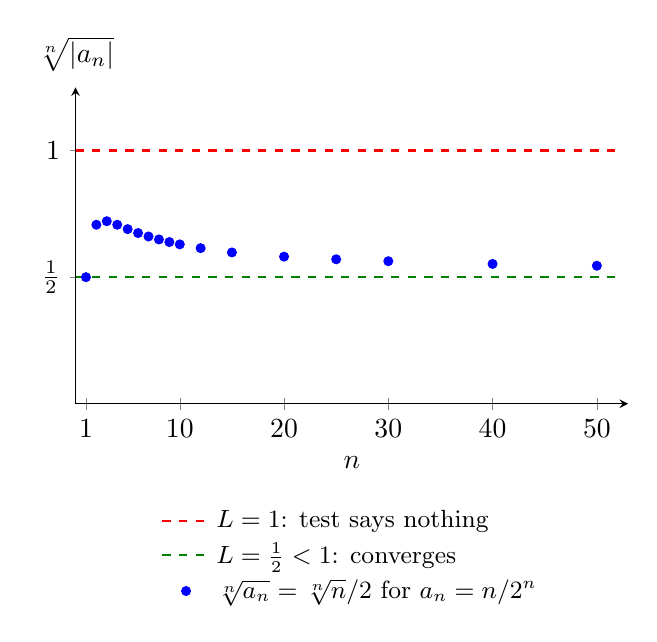
\begin{tikzpicture}
	\begin{axis}[
		axis lines=left,
		xmin=0, xmax=53, ymin=0, ymax=1.25,
		xtick={1,10,20,30,40,50}, ytick={0.5,1}, yticklabels={$\tfrac12$,$1$},
		xlabel={$n$}, ylabel={$\sqrt[n]{|a_n|}$},
		ylabel style={rotate=-90, anchor=south, at={(axis description cs:0,1.02)}},
		width=8.6cm, height=5.6cm, clip=false,
		legend style={at={(0.5,-0.3)}, anchor=north, draw=none, fill=none, font=\small}, legend cell align=left
		]
		\addplot[red, dashed, thick, domain=0:52, samples=2] {1};
		\addlegendentry{$L=1$: test says nothing}
		\addplot[green!50!black, dashed, thick, domain=0:52, samples=2] {0.5};
		\addlegendentry{$L=\tfrac12<1$: converges}
		\addplot[only marks, blue, mark=*, mark size=1.6pt] coordinates {(1,0.5) (2,0.7071) (3,0.7211) (4,0.7071) (5,0.6899) (6,0.6743) (7,0.6607) (8,0.6490) (9,0.6388) (10,0.6295) (12,0.6146) (15,0.5976) (20,0.5811) (25,0.5706) (30,0.5631) (40,0.5523) (50,0.5451)};
		\addlegendentry{$\sqrt[n]{a_n}=\sqrt[n]{n}/2$ for $a_n=n/2^n$}
	\end{axis}
\end{tikzpicture}
\end{document}
